% Scree plot: explained variance per principal component.
% Usage: % Scree plot: explained variance per principal component.
% Usage: % Scree plot: explained variance per principal component.
% Usage: % Scree plot: explained variance per principal component.
% Usage: \input{figures/scree-plot}
% Scale: x = 1 cm per PC (3 PCs), y = 6 cm per unit EVR (0..1.0 -> 0..6 cm)
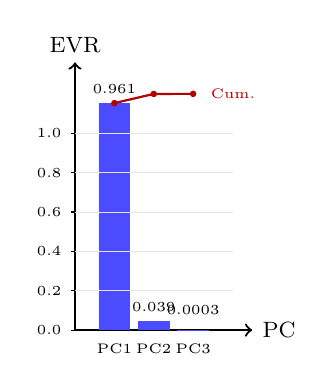
\begin{tikzpicture}[scale=0.5]
    % Axes
    \draw[thick, ->] (0,0) -- (4.5,0) node[right] {\footnotesize PC};
    \draw[thick, ->] (0,0) -- (0,6.8) node[above] {\footnotesize EVR};

    % Y-axis ticks
    \foreach \y/\ylab in {0/0.0, 1/0.2, 2/0.4, 3/0.6, 4/0.8, 5/1.0} {
        \draw (0,\y) -- (-0.1,\y);
        \node[left] at (-0.1,\y) {\tiny \ylab};
    }
    % X-axis labels
    \foreach \x/\xlab in {1/PC1, 2/PC2, 3/PC3} {
        \node[below] at (\x, -0.1) {\tiny \xlab};
    }

    % Bars: EVR = 0.9608, 0.0389, 0.0003 (scaled by 6)
    % PC1
    \fill[blue!70] (0.6, 0) rectangle (1.4, 5.765);
    \node[above] at (1.0, 5.765) {\tiny 0.961};
    % PC2
    \fill[blue!70] (1.6, 0) rectangle (2.4, 0.233);
    \node[above] at (2.0, 0.233) {\tiny 0.039};
    % PC3 (tiny, but still drawn)
    \fill[blue!70] (2.6, 0) rectangle (3.4, 0.002);
    \node[above] at (3.0, 0.15) {\tiny 0.0003};

    % Cumulative line (optional, shows the "knee")
    % Cumulative: 0.9608, 0.9997, 1.0000 (scaled by 6)
    \draw[thick, red!70!black, mark=*, mark size=1.5pt] plot coordinates {
        (1.0, 5.765) (2.0, 5.998) (3.0, 6.000)
    };
    \node[red!70!black, right] at (3.2, 6.0) {\tiny Cum.};

    % Grid lines (light)
    \foreach \y in {1,2,3,4,5} {
        \draw[gray!20, very thin] (0,\y) -- (4.0,\y);
    }
\end{tikzpicture}
% Scale: x = 1 cm per PC (3 PCs), y = 6 cm per unit EVR (0..1.0 -> 0..6 cm)
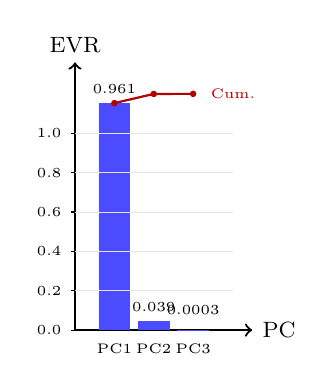
\begin{tikzpicture}[scale=0.5]
    % Axes
    \draw[thick, ->] (0,0) -- (4.5,0) node[right] {\footnotesize PC};
    \draw[thick, ->] (0,0) -- (0,6.8) node[above] {\footnotesize EVR};

    % Y-axis ticks
    \foreach \y/\ylab in {0/0.0, 1/0.2, 2/0.4, 3/0.6, 4/0.8, 5/1.0} {
        \draw (0,\y) -- (-0.1,\y);
        \node[left] at (-0.1,\y) {\tiny \ylab};
    }
    % X-axis labels
    \foreach \x/\xlab in {1/PC1, 2/PC2, 3/PC3} {
        \node[below] at (\x, -0.1) {\tiny \xlab};
    }

    % Bars: EVR = 0.9608, 0.0389, 0.0003 (scaled by 6)
    % PC1
    \fill[blue!70] (0.6, 0) rectangle (1.4, 5.765);
    \node[above] at (1.0, 5.765) {\tiny 0.961};
    % PC2
    \fill[blue!70] (1.6, 0) rectangle (2.4, 0.233);
    \node[above] at (2.0, 0.233) {\tiny 0.039};
    % PC3 (tiny, but still drawn)
    \fill[blue!70] (2.6, 0) rectangle (3.4, 0.002);
    \node[above] at (3.0, 0.15) {\tiny 0.0003};

    % Cumulative line (optional, shows the "knee")
    % Cumulative: 0.9608, 0.9997, 1.0000 (scaled by 6)
    \draw[thick, red!70!black, mark=*, mark size=1.5pt] plot coordinates {
        (1.0, 5.765) (2.0, 5.998) (3.0, 6.000)
    };
    \node[red!70!black, right] at (3.2, 6.0) {\tiny Cum.};

    % Grid lines (light)
    \foreach \y in {1,2,3,4,5} {
        \draw[gray!20, very thin] (0,\y) -- (4.0,\y);
    }
\end{tikzpicture}
% Scale: x = 1 cm per PC (3 PCs), y = 6 cm per unit EVR (0..1.0 -> 0..6 cm)
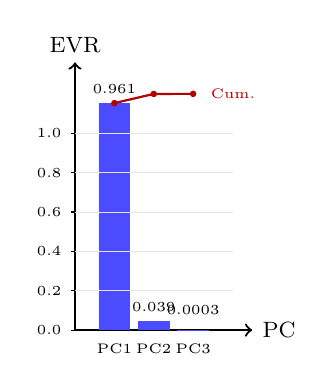
\begin{tikzpicture}[scale=0.5]
    % Axes
    \draw[thick, ->] (0,0) -- (4.5,0) node[right] {\footnotesize PC};
    \draw[thick, ->] (0,0) -- (0,6.8) node[above] {\footnotesize EVR};

    % Y-axis ticks
    \foreach \y/\ylab in {0/0.0, 1/0.2, 2/0.4, 3/0.6, 4/0.8, 5/1.0} {
        \draw (0,\y) -- (-0.1,\y);
        \node[left] at (-0.1,\y) {\tiny \ylab};
    }
    % X-axis labels
    \foreach \x/\xlab in {1/PC1, 2/PC2, 3/PC3} {
        \node[below] at (\x, -0.1) {\tiny \xlab};
    }

    % Bars: EVR = 0.9608, 0.0389, 0.0003 (scaled by 6)
    % PC1
    \fill[blue!70] (0.6, 0) rectangle (1.4, 5.765);
    \node[above] at (1.0, 5.765) {\tiny 0.961};
    % PC2
    \fill[blue!70] (1.6, 0) rectangle (2.4, 0.233);
    \node[above] at (2.0, 0.233) {\tiny 0.039};
    % PC3 (tiny, but still drawn)
    \fill[blue!70] (2.6, 0) rectangle (3.4, 0.002);
    \node[above] at (3.0, 0.15) {\tiny 0.0003};

    % Cumulative line (optional, shows the "knee")
    % Cumulative: 0.9608, 0.9997, 1.0000 (scaled by 6)
    \draw[thick, red!70!black, mark=*, mark size=1.5pt] plot coordinates {
        (1.0, 5.765) (2.0, 5.998) (3.0, 6.000)
    };
    \node[red!70!black, right] at (3.2, 6.0) {\tiny Cum.};

    % Grid lines (light)
    \foreach \y in {1,2,3,4,5} {
        \draw[gray!20, very thin] (0,\y) -- (4.0,\y);
    }
\end{tikzpicture}
% Scale: x = 1 cm per PC (3 PCs), y = 6 cm per unit EVR (0..1.0 -> 0..6 cm)
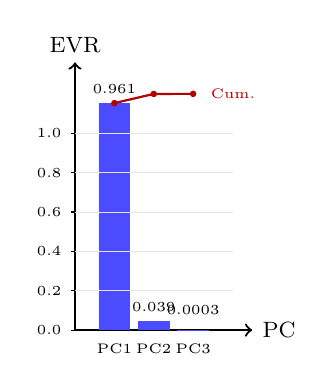
\begin{tikzpicture}[scale=0.5]
    % Axes
    \draw[thick, ->] (0,0) -- (4.5,0) node[right] {\footnotesize PC};
    \draw[thick, ->] (0,0) -- (0,6.8) node[above] {\footnotesize EVR};

    % Y-axis ticks
    \foreach \y/\ylab in {0/0.0, 1/0.2, 2/0.4, 3/0.6, 4/0.8, 5/1.0} {
        \draw (0,\y) -- (-0.1,\y);
        \node[left] at (-0.1,\y) {\tiny \ylab};
    }
    % X-axis labels
    \foreach \x/\xlab in {1/PC1, 2/PC2, 3/PC3} {
        \node[below] at (\x, -0.1) {\tiny \xlab};
    }

    % Bars: EVR = 0.9608, 0.0389, 0.0003 (scaled by 6)
    % PC1
    \fill[blue!70] (0.6, 0) rectangle (1.4, 5.765);
    \node[above] at (1.0, 5.765) {\tiny 0.961};
    % PC2
    \fill[blue!70] (1.6, 0) rectangle (2.4, 0.233);
    \node[above] at (2.0, 0.233) {\tiny 0.039};
    % PC3 (tiny, but still drawn)
    \fill[blue!70] (2.6, 0) rectangle (3.4, 0.002);
    \node[above] at (3.0, 0.15) {\tiny 0.0003};

    % Cumulative line (optional, shows the "knee")
    % Cumulative: 0.9608, 0.9997, 1.0000 (scaled by 6)
    \draw[thick, red!70!black, mark=*, mark size=1.5pt] plot coordinates {
        (1.0, 5.765) (2.0, 5.998) (3.0, 6.000)
    };
    \node[red!70!black, right] at (3.2, 6.0) {\tiny Cum.};

    % Grid lines (light)
    \foreach \y in {1,2,3,4,5} {
        \draw[gray!20, very thin] (0,\y) -- (4.0,\y);
    }
\end{tikzpicture}